\subsubsection{Description}

The virtual library permits to create a cell and map it to different libraries without having to change it.
    
\subsubsection{List of the generators provided}

\begin{itemize}
    \item \verb-a2- : \verb-q <= i0 & i1-
    \item \verb-a3- : \verb-q <= i0 & i1 & i2-
    \item \verb-a4- : \verb-q <= i0 & i1 & i2 & i3-
    \item \verb-na2- : \verb-nq <= ~ ( i0 & i1 )-
    \item \verb-na3- : \verb-nq <= ~ ( i0 & i1 & i2 )-
    \item \verb-na4- : \verb-nq <= ~ ( i0 & i1 & i2 & i3 )-
    \item \verb-o2- : \verb-q <= i0 & i1-
    \item \verb-o3- : \verb-q <= i0 & i1 & i2-
    \item \verb-o4- : \verb-q <= i0 & i1 & i2 & i3-
    \item \verb-no2- : \verb-nq <= ~ ( i0 & i1 )-
    \item \verb-no3- : \verb-nq <= ~ ( i0 & i1 & i2 )-
    \item \verb-no4- : \verb-nq <= ~ ( i0 & i1 & i2 & i3 )-
    \item \verb-inv- : \verb-nq <= ~ i-
    \item \verb-buf- : \verb-q <= i-
    \item \verb-xr2- : \verb-q <= i0 ^ i1-
    \item \verb-nxr2- : \verb-nq <= ~ ( i0 ^ i1 )-
    \item \verb-zero- : \verb-nq <= '0'-
    \item \verb-one- : \verb-q <= '1'-
    \item \verb-halfadder- : \verb-sout <= a ^ b- and \verb-cout <= a & b-
    \item \verb-fulladder- : \verb-sout <= a ^ b ^ cin-\\\indent and \verb-cout <= ( a & b ) | ( a & cin ) | ( b & cin )-
    \item \verb-mx2- : \verb-q <= (i0 & ~cmd) | (i1 & cmd)-
    \item \verb-nmx2- : \verb-nq <= ~( (i0 & ~cmd) | (i1 & cmd) )-
    \item \verb-sff- : \verb-if RISE ( ck ) : q <= i-
    \item \verb-sff2- : \verb-if RISE ( ck ) : q <= (i0 & ~cmd) | (i1 & cmd)-
    \item \verb-sff3- : \verb-if RISE ( ck ) :-\\\verb- q <= (i0 & ~cmd0) | (((i1 & cmd1)|(i2&~cmd1)) & cmd0)-
    \item \verb-ts- : \verb-if cmd : q <= i-
    \item \verb-nts- : \verb-if cmd : nq <= ~i-
\end{itemize}

\subsubsection{Mapping file}

The virtual library is mapped to the sxlib library. A piece of the corresponding mapping file is shown below.\\
\indent In order to map the virtual library to another library, on has to write a .xml file which makes correspond models and interfaces.\\
\indent Note that the interfaces of the cells must be the same (except for the names of the ports). Otherwise, one has to create .vst file in order to make the interfaces match.\\

\indent The environment variable used to point the right file is \verb-STRATUS_MAPPING_NAME-.

\begin{figure}[hbtp]
\centering
\latexhtml{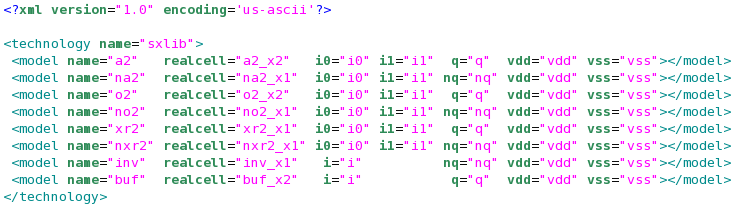
\includegraphics[width=\textwidth]{images/xml}}
          {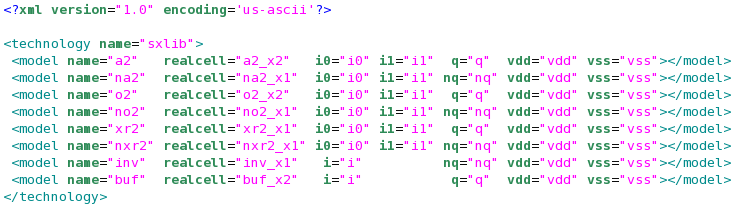
\includegraphics[width=\textwidth]{images/xml.png}}
\end{figure}

\subsubsection{Generators}

Some generators are also provided in order to use the cells of the library with nets of more than 1 bit. One has to upper the first letter of the model name in order to user those generators. What is simply done is a for loop with the bits of the nets. The parameter \verb-'nbit'- gives the size of the generator.

\subsubsection{Example}

\begin{itemize}
    \item Direct instanciation of a cell
\end{itemize}
\begin{verbatim}
for i in range ( 4 ) :
  Inst ( 'a2'
       , map = { 'i0'  : neti0[i]
               , 'i1'  : neti1[i]
               , 'q'   : netq[i]
               , 'vdd' : netvdd
               , 'vss' : netvss
               }
       )
\end{verbatim}

\begin{itemize}
    \item Instanciation of a generator
\end{itemize}
\begin{verbatim}
Generate ( 'A2', "my_and2_4bits", param = { 'nbit' : 4 } )
Inst ( 'my_and2_4bits'
     , map  = { 'i0'  : neti0
              , 'i1'  : neti1
              , 'q'   : netq
              , 'vdd' : vdd
              , 'vss' : vss
              }
     )
\end{verbatim}

\subsubsection{Errors}
    
Some errors may occur :
\begin{itemize}
    \item \verb-[Stratus ERROR] Inst : the model ... does not exist.-\\\verb-Check CRL_CATA_LIB.-\\The model of the cell has not been found. One has to check the environment variable.
    \item \verb-[Stratus ERROR] Virtual library : No file found in order to parse.-\\\verb-Check STRATUS_MAPPING_NAME.-\\The mapping file is not given in the environment variable.
\end{itemize} 

\begin{htmlonly}
\subsubsection{See Also}

\hyperref[ref]{\emph{Introduction}}{}{Introduction}{secintroduction}

\end{htmlonly}
